\section{Introduction and Overview}
\subsection{Research}

\subsection{Test environment}
A virtual network was set up on Azure-Cloud as a test environment. The test network was set up in the cloud so that the development team can access the network regardless of its location. The test network consists of a Windows server and two Windows clients. Active Directory service was configured on the server to manage the client computer. The following operating systems were installed in this testnetwork: \\
\\
\textbf{Server:}
\begin{itemize}
    \item Windows Server 2016
\end{itemize}
\textbf{Clients:}
\begin{itemize}
    \item Windows 10 Pro, Version 1709
\end{itemize}
The network is structured as followed:\\
\begin{figure}[H]
    \centering
    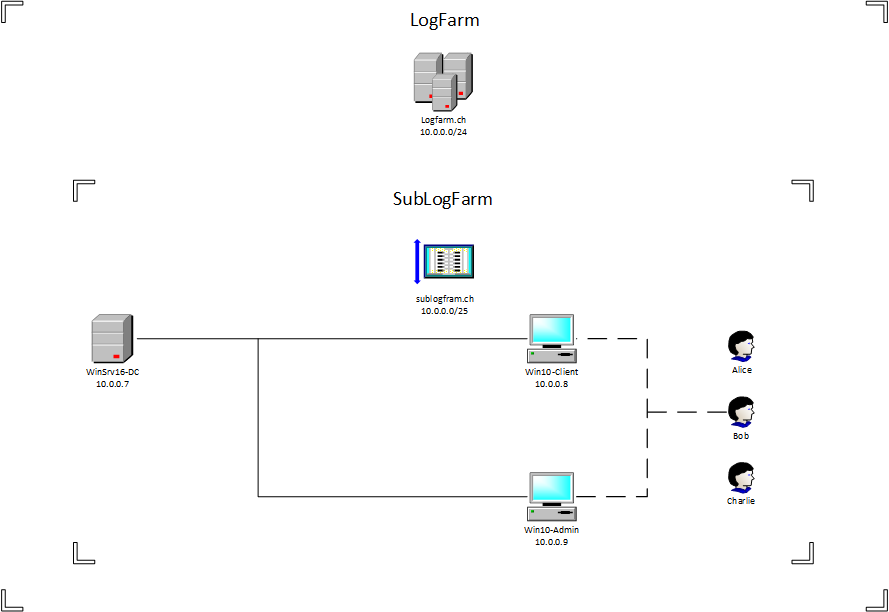
\includegraphics[width=0.9\linewidth]{assets/testnetwork.png}
    \caption{test environment}
\end{figure}
\subsubsection{Users}
Three different users were configured:
\begin{table}[H]
    \centering
    \begin{tabular}{p{4cm} p{8cm}} \hline
        \textbf{Name} & \textbf{Permissions}  \\ \hline
        alice & administration  \\ \hline
        bob & user  \\ \hline
        charlie & user  \\ \hline
    \end{tabular}
    \caption{Angaben Lukas Kellenberger}
\end{table}